\section{Résultats et Comparaisons}
\subsection{Résultats du papier}
% Toutes les images avec l'algorihtme du point fixe

Dans cette section, nous présentons uniquement les résultats graphiques obtenus à l'aide de la méthode du point fixe \eqref{pt_fixe} sur les exemples du papier. Les figures sont affichées dans l'ordre chronologique d'obtention, afin de suivre l'évolution de la flexibilité de notre code. Un court commentaire accompagne chaque image afin de mettre en évidence les aspects notables du résultat obtenu, ainsi que les difficultés rencontrées. Nous donnons des informations complémentaires avec chaque visualisation, telles que le nombre $n$ d'itérations nécessaires à la convergence ou l'erreur $\varepsilon$ en norme L1. Pour calculer les erreurs nous avons trouvé nous-mêmes les formes analytiques de chacune des fonctions solutions qui, contrairement aux intensités lumineuses n'étaient pas données dans le papier.

\subsubsection{Les paraboles}
Les premières figures présentées dans notre papier étaient deux paraboles à bases carrées définies sur  $\omb = \ff{0,1}\times \ff{0,1}$. Nous avons fait le choix d'initialiser l'algorithme avec $U^0 = 0$ sur $\omb$.
\vspace{1em}
% insert an image as wide as 70% of line length
\begin{figure}[!htb]
    \centering
    \fbox{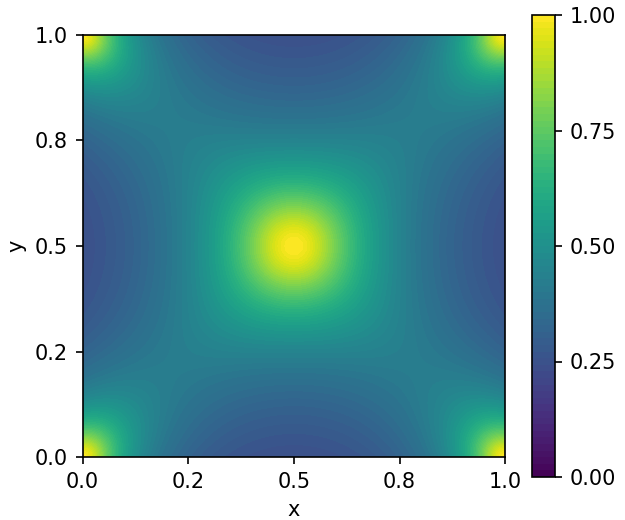
\includegraphics[width=.48\linewidth]{./Images/int_parabole.png}}

    \vspace{0.5em}

    % Légende centrée "Figure X – ..."
    \refstepcounter{figure} % incrémente le compteur de figure
    \centering
    \text{Figure~\thefigure{} – Intensité lumineuse,}
    % Équation centrée juste en dessous
    \[
        I(x, y) = \frac{1}{
            \sqrt{1 + \left(16y(1 - y)(1 - 2x)\right)^2 + \left(16x(1 - x)(1 - 2y)\right)^2}
        }.
    \]
    \label{Fig:int_parabole}
\end{figure}
% insert 2 side by side redimensionned images
\begin{figure}[!htb]
    \begin{minipage}[t]{0.48\textwidth}
        \centering
        \fbox{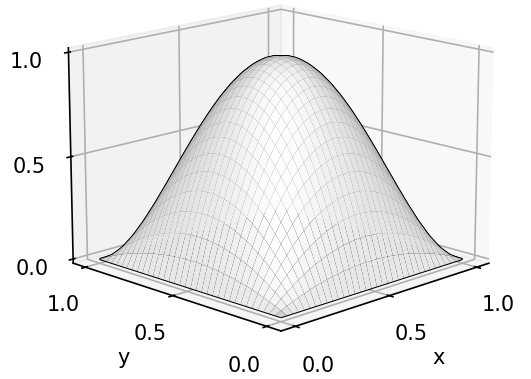
\includegraphics[width=.9\linewidth]{./Images/parabole.png}}
        \caption{Parabole, $101\times101 $ points,\\[0.8ex] \centering$\varepsilon=6.34 \times 10^{-3}$, $n=1730$, $u\left( 
            \dfrac{1}{2},\dfrac{1}{2} \right)=1$.}\label{Fig:parabole}
    \end{minipage}\hfill
    \begin{minipage}[t]{0.48\textwidth}
        \centering
        \fbox{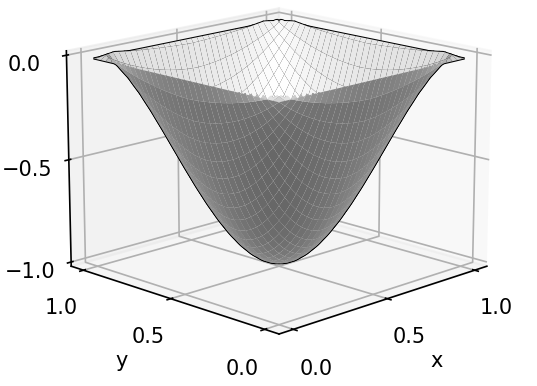
\includegraphics[width=.9\linewidth]{./Images/reverse_parabole.png}}
        \vspace{0.9em}

        % Légende centrée "Figure X – ..."
        \refstepcounter{figure} % incrémente le compteur de figure
        \centering
        \text{Figure~\thefigure{} – Parabole renversée,}\\[0.5em]
        \text{$101 \times 101$ points, $\varepsilon=1.7\times 10^{-2}$, $n=100$,}
        \[
            u\left( \dfrac{1}{2},\dfrac{1}{2}\right) = -1.
        \]\label{Fig:reverse_parabole}
    \end{minipage}
\end{figure}
\newpage
Cet exemple illustre parfaitement le problème d'unicité du problème. En effet, pour une même intensité lumineuse donnée, nous obtenons deux formes différentes en ayant modifié l'information de $u\left(\frac{1}{2},\frac{1}{2} \right)$.

La différence du nombre d'itération nécessaires à la convergence entre les deux figures est flagrante. Nous avons donc cherché une solution pour optimiser le temps de convergence. Nous nous sommes alors rendu compte qu'en modifiant le $U^0$ initial, nous pouvions drastiquement réduire le nombre d'itération. En choisissant $U^0=0$ sur $\p \omb$ et $U^0=1$ dans $\Omega$ nous avons obtenu pour la \textit{Parabole} $n=85$, et $n=100$ pour la \textit{Parabole renversée}. 
Nous pouvons aussi noter une légère différence pour l'erreur, mais nous n'avons pas réussi à déterminer d'où venait cet écart.

\subsubsection{La pyramide}
La \textit{Pyramide} fut le second exemple donné dans le papier. Ici encore, $\omb = \ff{0,1}\times \ff{0,1}$ et nous avons initialisé avec $U^0 = 0$ sur $\omb$. 
\begin{noremark}
    Utiliser le $U^0$ optimal précédent ne change rien à la convergence pour cette figure.
\end{noremark}

% insert 2 side by side redimensionned images
\begin{figure}[!htb]
    \begin{minipage}[t]{0.48\textwidth}
        \centering
        \fbox{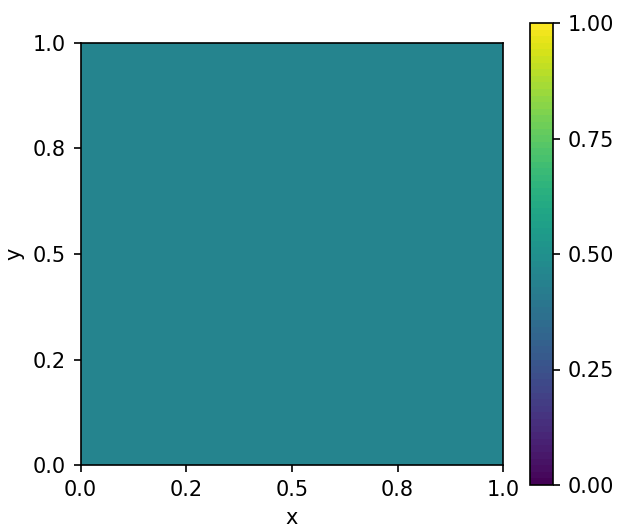
\includegraphics[width=.9\linewidth,height=5.5cm]{./Images/int_pyramide.png}}
        \caption{Intensité lumineuse,  \centering $I(x,y)=\dfrac{1}{\sqrt{5}}.$}\label{Fig:int_pyramide}
    \end{minipage}\hfill
    \begin{minipage}[t]{0.48\textwidth}
        \centering
        \fbox{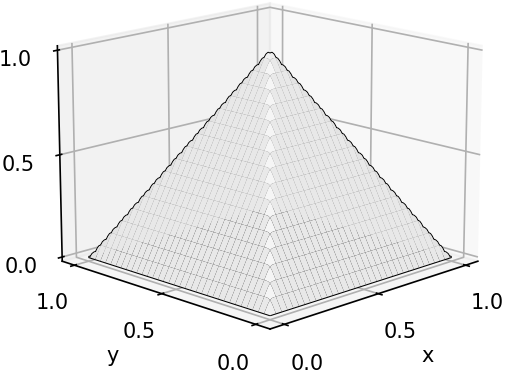
\includegraphics[width=.9\linewidth,height=5.5cm]{./Images/pyramide.png}}
        \caption{Pyramide, $101\times101 $ points, \\[1ex] \centering$\varepsilon=1.65 \times 10^{-4}$, $n=100$.}\label{Fig:pyramide}
    \end{minipage}
\end{figure}
\newpage
Cette figure est particulière. En effet, celle-ci ne possède aucun point d'intensité égale à $1$. D'après ce qui précède, la solution est donc unique. Nous n'avons donc pas besoin de fixer des valeurs à l'intérieur de la grille pour s'assurer de la convergence vers \og la bonne solution \fg.

\subsubsection{Deux autres exemples}
Dans cette dernière sous-section, nous présentons deux exemples illustrant la sensibilité du processus de reconstruction par rapport aux données internes de la grille. Nous avons $\omb = \ff{0,1}\times \ff{0,1}$ et $U^0$ est choisi comme le $U^0$ optimisé des paraboles.

% insert an image as wide as 70% of line length
\begin{figure}[!htb]
    \centering
    \fbox{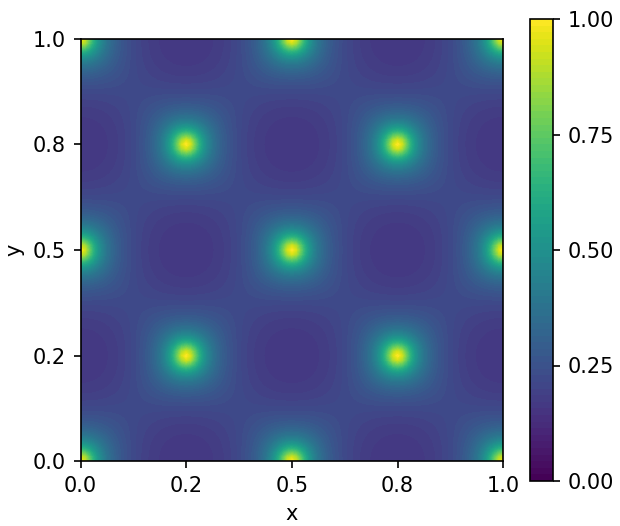
\includegraphics[width=.48\linewidth]{./Images/int_fig78.png}}
    \vspace{0.5em}

    % Légende centrée "Figure X – ..."
    \refstepcounter{figure} % incrémente le compteur de figure
    \centering
    \text{Figure~\thefigure{} – Intensité lumineuse,}
    % Équation centrée juste en dessous
    \[
        I(x, y) = \frac{1}{
            \sqrt{1 + \left(2\pi\sin(2\pi y)\cos(2\pi x)\right)^2 + \left(2\pi\sin(2\pi x)\cos(2\pi y)\right)^2}
        }.
    \]
\end{figure}
\vspace{10cm} % Espacement réduit ici si besoin
% insert 2 side by side redimensionned images
\begin{figure}[!htb]
    \begin{minipage}[t]{0.48\textwidth}
        \centering
        \fbox{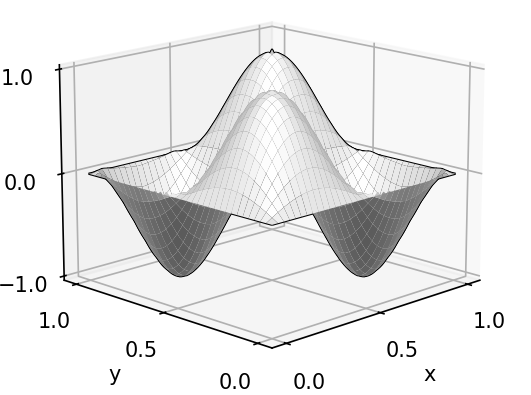
\includegraphics[width=.9\linewidth,height=5.5cm]{./Images/fig7.png}}
        \caption{
            $101\times101 $ points, \\[0.5em] \centering$\varepsilon=6.34\times10^{-3}$, $n = 110$,
            \centering\protect
            $\begin{aligned}
                    u\left(\dfrac{1}{4},\dfrac{3}{4} \right) &= u\left(\dfrac{3}{4},\dfrac{1}{4} \right) = -1, \\
                    u\left(\dfrac{1}{4},\dfrac{1}{4} \right) &= u\left(\dfrac{3}{4},\dfrac{3}{4} \right) = 1, \\
                    u\left(\dfrac{1}{2},\dfrac{1}{2} \right) &= 0.
                \end{aligned}$
        }\label{Fig:fig7}
    \end{minipage}\hfill
    \begin{minipage}[t]{0.48\textwidth}
    \centering\fbox{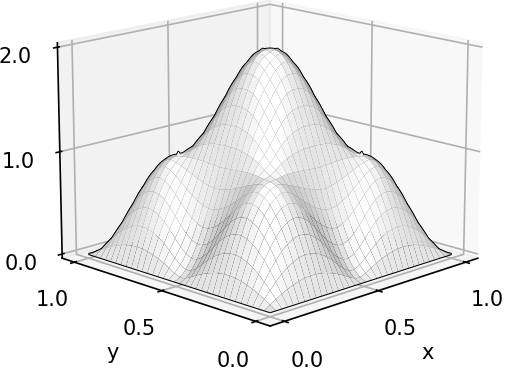
\includegraphics[width=.9\linewidth,height=5.5cm]{./Images/fig8.png}}
        \caption{
            $101\times101 $ points, $n=350,$\\[1ex]
            \centering\protect
            $\begin{aligned}
                u\left(\dfrac{1}{4},\dfrac{3}{4} \right) &= u\left(\dfrac{3}{4},\dfrac{1}{4} \right) = 1, \\
                u\left(\dfrac{1}{4},\dfrac{1}{4} \right) &= u\left(\dfrac{3}{4},\dfrac{3}{4} \right) = 1, \\
                u\left(\dfrac{1}{2},\dfrac{1}{2} \right) &= 2.
            \end{aligned}$
        }\label{Fig:fig8}
    \end{minipage}
\end{figure}


Sur l'intensité lumineuse nous remarquons $5$ points intérieurs d'intensité $1$. Encore une fois, nous devons connaître la hauteur en ces points de la solution pour s'assurer de converger vers la bonne solution étudiée. Nous avons essayé de trouver la solution analytique de la Figure \ref{Fig:fig8} afin de calculer l'erreur. En faisant de grandes intégrations de l'intensité, nous n'avons malheureusement pas trouvé cette solution. C'est pourquoi celle-ci manque à la légende de la  figure. 

\begin{noremark}
    Nous nous sommes rendu compte plus tard que dans le papier de Mme Rouy et Mme Tourin, aucune erreur n'était donnée pour cette figure. Nous en avons déduit qu'elles n'avaient pas réussi non plus à déterminer la solution analytique.
\end{noremark}

\subsection{Résultats supplémentaires}
Dans cette section, nous présentons des résultats complémentaires à ceux donnés dans le papier. En retrouvant au fur et à mesure les figures du papier, nous avons eu l'envie de jouer avec notre code et de tester ses limites. 

Contrairement aux exemples de la section précédente, nous avons ici adopté une approche différente. En effet, l’intensité lumineuse des courbes que nous souhaitions reconstituer n’était pas connue à l’avance. Plutôt que de partir de la lumière renvoyée par l’objet pour en déduire sa forme (comme nous l’avions fait auparavant) nous avons inversé la démarche : à partir de la forme de l’objet, nous avons calculé son gradient afin d’estimer l’intensité lumineuse qu’il renvoie. Cette intensité a ensuite été transmise à notre programme, qui a alors tenté de retrouver la courbure de l’objet initial.

Puisque nous partions des solutions analytiques, nous avons pu calculer l'erreur en norme L1 pour les deux figures que nous allons présenter.


\subsubsection{La demi-parabole}
Jusqu’à présent, nous nous sommes uniquement intéressés à des cas où les formes étudiées possédaient un nombre fini de points critiques. Afin d’évaluer l’influence éventuelle de ce caractère fini sur la qualité de la reconstruction, nous avons cherché à analyser une courbe présentant une infinité de points d’intensité lumineuse égale à 1. L’objectif était de déterminer si le fait que les points critiques soient en nombre dénombrable dans les exemples précédents jouait un rôle dans les performances de notre méthode.

Nous avons alors pensé la fonction $f(x,y) = x^2$ dans $\R^2$. En effet, celle-ci possède un nombre indénombrable de points critiques sur l'axe $x=0$. Nous avons travaillé dans $\omb = \ff{-1,1}\times \ff{-1,1}$ et choisi, $U^0=1$ sur les axes $x=-1$ et $x=1$. Les autres bords sont $U^0=x^2$ sur les axes $y=-1$ et $y=1$. Enfin, dans $\Omega'$, $U^0=0$.

\begin{figure}[!htb]
    \centering
    \begin{minipage}[t]{0.48\textwidth}
        \centering
        \fbox{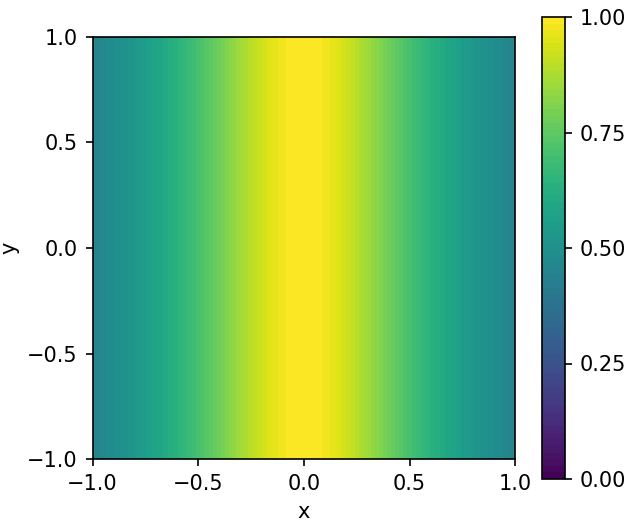
\includegraphics[width=.9\linewidth,height=5.5cm]{./Images/int_x2.png}}
        \caption{Intensité lumineuse,\\[1ex] \centering $I(x,y)=\dfrac{1}{\sqrt{1+{(2x)}^2}}.$}
        \label{Fig:int_x2}
    \end{minipage}%
    \hfill
    \begin{minipage}[t]{0.48\textwidth}
        \centering
        \fbox{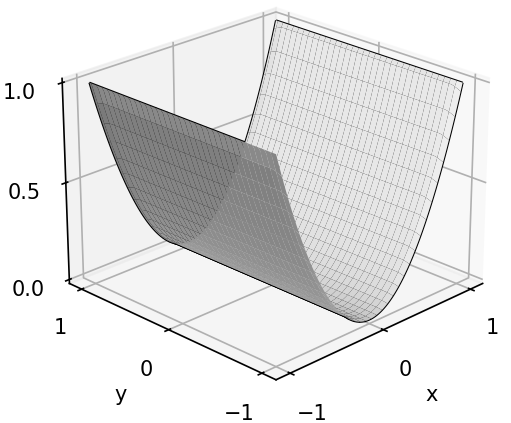
\includegraphics[width=.9\linewidth,height=5.5cm]{./Images/x2.png}}
        \vspace{0.9em}

        % Légende centrée "Figure X – ..."
        \refstepcounter{figure} % incrémente le compteur de figure
        \centering
        \text{Figure~\thefigure{} – $f(x,y)=x^2$,}\\[0.5em]
        \text{$101 \times 101$ points, $\varepsilon=9.75\times 10^{-3}$, $n=80$,}
        \[
            u\big|_{x=0} = 0.
        \]\label{Fig:x2}
    \end{minipage}
\end{figure}

Cet exemple illustre bien le fait que le nombre de points critiques n'est pas un problème pour le schéma numérique. 
Nous avons fait tendre le pas du schéma vers 0 et nous n'avons constaté aucun problème de convergence particulier vers la solution de viscosité. 
\begin{noremark}
    En modifiant les conditions aux bords nous avons aussi réussi à faire converger le programme vers des solutions de viscosités qui avaient perdu leur caractère $C^1$. Nous donnons un exemple de celles-ci en dessous avec $U^0=0$ sur les bords.
\end{noremark}
\vspace{10cm} % Espacement réduit ici si besoin
% insert an image as wide as 70% of line length
\begin{figure}[htb]
    \centering
    \fbox{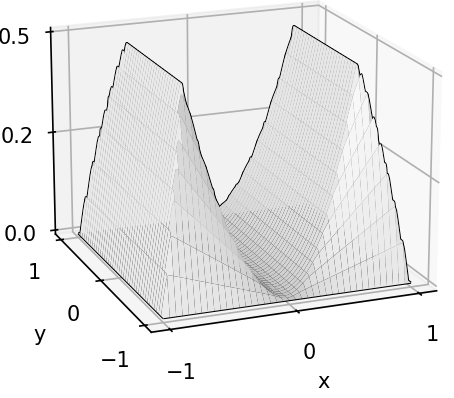
\includegraphics[width=.48\linewidth]{./Images/x2_mixedbd.png}}
    \caption{$101\times 101$ points, $n=275$,  $\left. u\right|_{x=0}=0.$ }\label{Fig:x2_mixedbd}
\end{figure}


\subsubsection{Le vase}
Après avoir étudié un cas présentant une infinité de points critiques, nous avons entrepris la reconstitution d’un \textit{Vase}. Cet objet, plus complexe que les courbes précédemment analysées. Il nous a servis de source de motivation et de compréhension, car c’est en travaillant sur cette forme que nous avons véritablement assimilé les principes du Shape-from-Shading.

Nous avons choisi de présenter cet exemple en dernier, car il s’agit de la forme la plus difficile que nous ayons eu à traiter. Elle constitue à la fois un défi technique et une illustration de l’efficacité de notre méthode. Nous donnons l'intensité lumineuse du \textit{Vase} ainsi que les images de sa reconstruction sous deux angles différents avant de rentrer dans les détails de la complexité.

\begin{figure}[htb]
    \centering
    \fbox{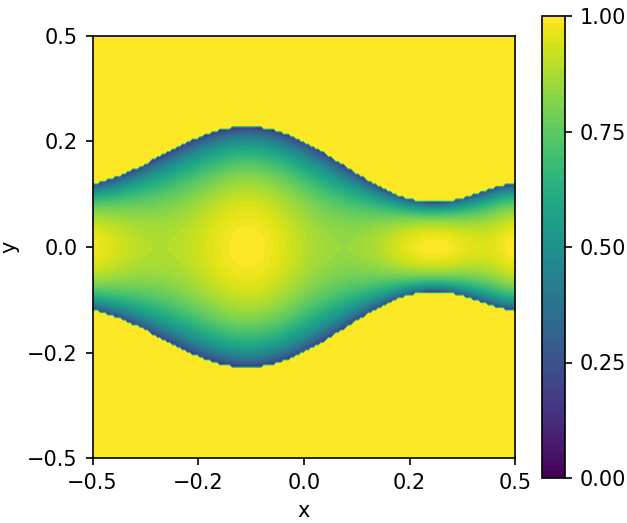
\includegraphics[width=.5\linewidth]{./Images/int_vase.png}}
    \caption{Intensité lumineuse du vase.}\label{Fig:int_vase}
\end{figure}
\vspace{15cm} % Espacement réduit ici si besoin
% insert 2 side by side redimensionned images
\begin{figure}[!htb]
    \begin{minipage}[t]{0.48\textwidth}
        \centering
        \fbox{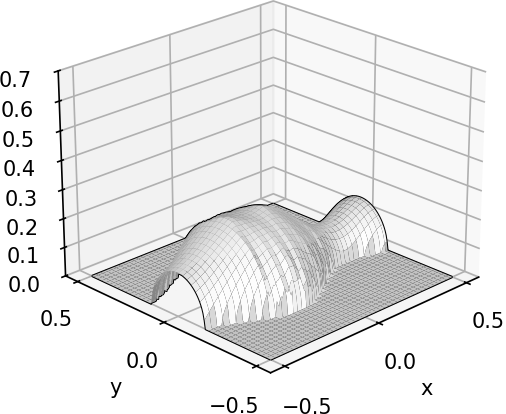
\includegraphics[width=.9\linewidth,height=5.5cm]{./Images/vase_cote.png}}
        \caption{Vase vu de côté.}\label{Fig:vase_cote}
    \end{minipage}\hfill
    \begin{minipage}[t]{0.48\textwidth}
    \centering\fbox{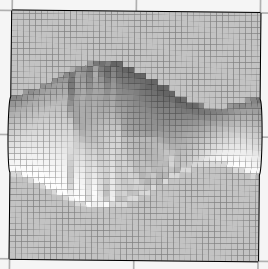
\includegraphics[width=.8\linewidth,height=5.5cm]{./Images/vase_dessus.png}}
        \caption{Vase vu du dessus.}\label{Fig:vase_dessus}
    \end{minipage}
\end{figure}

Pour les deux figures, nous avons travaillé sur $\omb=\ff{-0.5,0.5}\times \ff{-0.5,0.5}$ avec\\ $171\times 171$ points. L'erreur en norme L1 est de $4.12 \times 10^{-3}$ et il a fallu 220 itérations pour converger. 

Nous allons à présent développer les difficultés rencontrées quant à la reconstruction du \textit{Vase}. Nous avons dans un premier temps trouvé l'équation d'un vase en 2D. Sur internet nous avons trouvé l'équation suivante sur $\ff{-0.5,0.5}\times \ff{-0.5,0.5}$
\begin{align}
    vase(x,y) =\left\{
    \begin{array}{ll}
         \mathopen{}\sqrt{P(x)^2 -y^2} & \ \text{si } P(x)^2-y^2>0\\  
         0& \ \text{sinon }
    \end{array}
    \right.
\end{align}
où $P(x) = 0.15 - 0.025(6x- 1) (2x - 1)^2 (3x + 2)^2 (2x + 1)$.

Nous avons ensuite calculé les dérivées partielles de cette fonction et en avons déduit l'intensité lumineuse de notre objet. Nous ne donnerons pas l'expression explicite de celle-ci. Nous avons alors longtemps bloqué sur la reconstruction, en effet, le \textit{Vase} ne recouvre pas le carré en entier. Ainsi, il a fallu donner des conditions aux bords différentes de celles qu'on utilisait précédemment. Nous avons donc dû donner au programme les valeurs exactes du \textit{Vase} sur les axes $x=-0.5$ et $x=0.5$ ainsi que sur les points intérieurs d'intensité 1. Il n'a pas été facile de lier toutes les conditions entre elles. 

Comme nous pouvons le constater sur la Figure \ref{Fig:int_vase}, il y a beaucoup de points ayant une intensité lumineuse proche de 1. Cela joue une importance particulière sur la reconstruction de la partie centrale du \textit{Vase} qui présente certaines imperfections (voir Figure \ref{Fig:vase_cote} et Figure \ref{Fig:vase_dessus}). En effet, puisque celui-ci est assez plat, de nombreuses erreurs d'arrondi ont lieu dans cette zone. Nous avons rencontré quelques difficultés liées à ces erreurs d'arrondi que nous avons donc dû gérer du mieux possible. Actuellement, notre programme met toujours beaucoup de temps à converger dans cette partie du \textit{Vase}.

\begin{noremark}
    Nous pouvons voir sur la Figure \ref{Fig:int_vase} que toute la partie en dehors du \textit{Vase} possède une intensité lumineuse égale à 1. C'est un choix de notre part. Il était plus facile pour nous de considérer cette zone externe comme une partie du \textit{Vase}, mais avec une hauteur de 0. En effet, nous aurions pu fixer l'intensité lumineuse du \textit{Vase} dans cette partie comme  \og NAN \fg{} (Not A Number) ce qui donnerait quelque chose de plus cohérent. Mais cela aurait engendré de gros changements dans notre code pour le même résultat. 
\end{noremark}



\subsection{Comparaison des algorithmes}
Tous les résultats présentés dans la section précédente ont été obtenus à l’aide du schéma explicite basé sur l’algorithme du point fixe. Nous souhaitons à présent mettre en évidence l’efficacité de l’algorithme \eqref{algo_papier} proposé dans l’article. Pour cela, nous allons comparer les deux méthodes en termes de nombre d’itérations nécessaires à la convergence, ainsi que de l’erreur relative entre les solutions obtenues avec \eqref{pt_fixe} et avec \eqref{algo_papier}. Nous n'allons pas revoir tous les exemples précédents. Nous avons sélectionné les exemples les plus pertinents illustrant la performance de l'algorithme du papier et mis les informations importantes dans un tableau que nous commenterons. 

Les trois exemples ci-dessous ont été retrouvés avec les mêmes conditions initiales qu'avant. Les intensités lumineuses sont aussi identiques à celles utilisées plus tôt dans notre rapport.
\begin{figure}[!htb]
    \centering
    \begin{minipage}[t]{0.48\textwidth}
        \centering
        \fbox{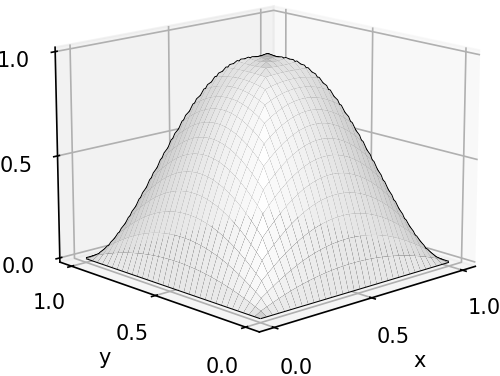
\includegraphics[width=.9\linewidth,height=5.5cm]{./Images/parabole_opti.png}}
        \caption{Parabole obtenue avec \\ \centering l'algorithme du papier, $101\times101$ points.}
        \label{Fig:parabole_opti}
    \end{minipage}%
    \hfill
    \begin{minipage}[t]{0.48\textwidth}
        \centering
        \fbox{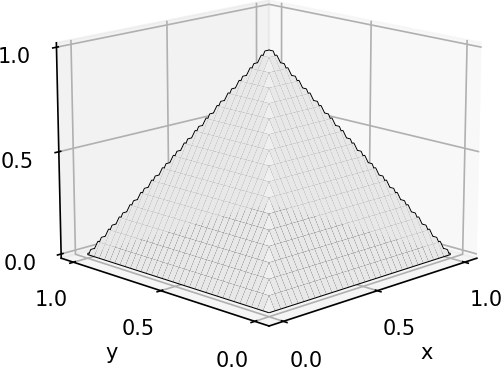
\includegraphics[width=.9\linewidth,height=5.5cm]{./Images/pyramide_opti.png}}
        \caption{Pyramide obtenue avec \\ \centering l'algorithme du papier, $101\times101$ points.}
        \label{Fig:pyramide_opti}
    \end{minipage}
\end{figure}
\begin{figure}[!ht]
\centering
    \begin{minipage}[t]{0.48\textwidth}
        \centering
        \fbox{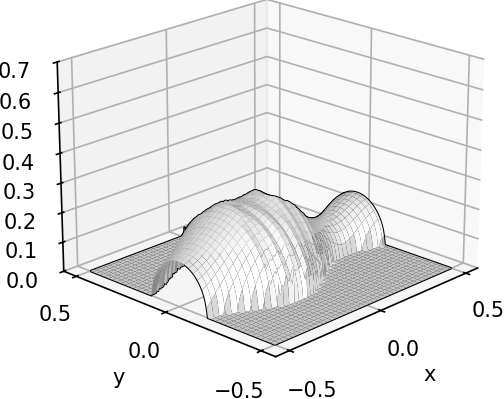
\includegraphics[width=.95\linewidth,height=5.5cm]{./Images/vase_opti.png}}
        \caption{Vase obtenu avec \\ \centering l'algorithme du papier, $171\times171$ points.}
        \label{Fig:vase_opti}
    \end{minipage}
\end{figure}

\begin{figure}[!htb] 
    \centering
    \renewcommand{\arraystretch}{1.5} % pour espacer verticalement
    \begin{tabular}{|c|c|c|c|c|}\hline
         & $\varepsilon$ point fixe & $\varepsilon$ algorithme & $n$ point fixe & $n$ algorithme \\ \hline
        Parabole & $6.34 \times 10^{-3}$ & $7.52 \times 10^{-3}$ & 85 & 48 \\ \hline
        Pyramide & $1.65 \times 10^{-4}$ & $1.16 \times 10^{-16}$ & 100 & 49\\ \hline
        Vase     & $4.12 \times 10^{-3}$ & $2.85 \times 10^{-3}$ & 220 & 90 \\  \hline
    \end{tabular}
    \caption{Comparaison du nombre d'itérations et de l'erreur pour les deux méthodes.}
    \label{fig:comparaison_algo}
\end{figure}

La première différence notable que l'on observe sur la figure \ref{Fig:parabole_opti} est l'apparence plus linéaire de la \textit{Parabole}. En effet, ses bords ainsi que son sommet sont bien moins arrondis que ceux de la \textit{Parabole} reconstruite avec \eqref{pt_fixe} (voir Figure \ref{Fig:parabole}). On peut d'ailleurs voir que cela se ressent en regardant l'erreur des deux paraboles. En effet, bien que l'algorithme \eqref{algo_papier} converge 1,7 fois plus vite, l'erreur en norme L1 de notre \textit{Parabole} est légèrement plus élevée ici que la première (Elles sont presque égales).

Pour la \textit{Pyramide}, nous observons à nouveau une différence graphique. Cependant, celle-ci est bien plus subtile que pour la \textit{Parabole}. En effet, à la place d'avoir des pentes presque lisses, celle-ci présente de légères \og marches d'escaliers \fg{} (voir Figure \ref{Fig:pyramide_opti}). En opposition à la \textit{Parabole}, la différence entre les deux erreurs est flagrante. En effet, l'erreur est $10^{12}$ fois plus petite pour l'algorithme du papier. Le nombre d'itérations nécessaires à la convergence est de seulement de $49$, soit deux fois moins que pour l'algorithme du point fixe. On comprend donc que pour la \textit{Pyramide}, l'algorithme \eqref{algo_papier} est en tout point plus performant.

Lorsque l'on reconstruit le \textit{Vase} avec notre algorithme, on observe que la convergence nécessite $2.4$ fois moins d'itérations qu'avec l'algorithme \eqref{pt_fixe}. Cependant, cela se produit au prix d'un résultat graphique moins esthétique. En effet, observe une certaine imperfection au niveau de la zone la plus haute du \textit{Vase}. Cela est encore du aux erreurs d'arrondis dans cette zone presque plate.

L'algorithme du papier est donc bien plus performant d'un point de vue itératif que l'algorithme du point fixe. Quand à l'erreur, elle est inférieure ou équivalente à celle du point fixe. On retiendra tout de même la capacité de \eqref{pt_fixe} à obtenir des résultats plus lisses et plus proches (visuellement parlant) du véritable objet.\\

Nous allons à présent illustrer un exemple sur lequel l'algorithme \eqref{algo_papier} ne fonctionne pas totalement. Il s'agit de la Figure $\ref{Fig:fig7}$. 
\begin{figure}[!ht]
\centering
    \begin{minipage}[t]{0.48\textwidth}
        \centering
        \fbox{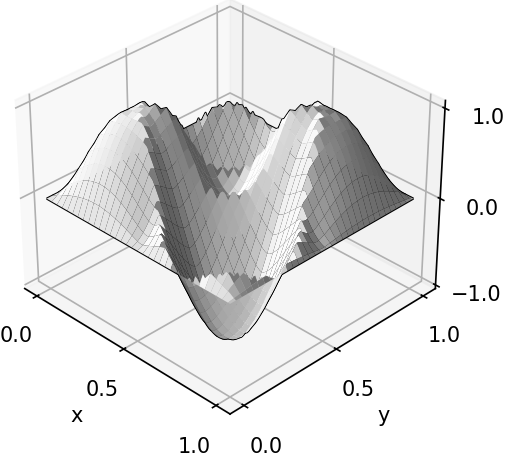
\includegraphics[width=.9\linewidth,height=5.5cm]{./Images/fig7_opti.png}}
        \caption{Mauvaise convergence obtenue avec l'algorithme du papier, \\[1ex] \centering  $101\times101$ points}
        \label{Fig:fig7_opti}
    \end{minipage}
\end{figure}
\newpage
Pour cette reconstruction, l'erreur est $9.83 \times 10^{-2}$ et l'algorithme a convergé en $50$ itérations. L'erreur est donc bien plus grande que celle obtenue avec la reconstruction par la méthode du point fixe (l'erreur était de $6.34 \times 10^{-3}$). Graphiquement parlant, on voit facilement d'où vient ce problème. En effet, les pentes des sommets ne sont pas bombées mais bien creuse. L'algorithme \eqref{algo_papier} semble ne pas réussir à approcher correctement cette partie de la Figure \ref{Fig:fig7_opti}.

\begin{noremark}
    Nous n'avons pas réussi à déterminer clairement pourquoi est-ce que l'algorithme \eqref{algo_papier} n'arrivait pas à converger dans ce cas-là. Il se pourrait que nous atteignions les limites de l'algorithme \eqref{algo_papier}. En effet, peut-être que la formule \og inventée \fg{} par ChatGPT n'est valable que dans certaines situations/hypothèses. \\ 
    Il se pourrait aussi que nous ayons une erreur dans notre code, mais cela serait assez surprenant car celui-ci fonctionne pour le reste des figures.
\end{noremark}




